\section{The design of the testing framework}\label{chp:testing-tool}

% First, we will start with the list of the specifications for the framework. Before we go through them one by one and look at the way that they are implemented in more detail we define some terms and explain the project structure.

% \subsection{The framework specifications}
    We will start by laying down the specifications for the implementation of \projectname:
    \begin{enumerate}
        \item execute registered logical attacks on a real physical JavaCard (see~\ref{sec:build-execute-attacks}),
        \item visualize the results of the attacks in a concise and clear manner (see~\ref{sec:visualization}),
        \item be extensible --- allow adding new attacks in the future (see~\ref{sec:attack-recipe}).
        \item be cross-platform, i.e. support at least Linux and Windows platforms (see~\ref{sec:invocation}),
    \end{enumerate}


    And we also introduce a new terminology, that will be used with few exceptions:

                \begin{enumerate}
                    \item[\textbf{attack}] is the overarching term used for describing a (particular) way of exploiting a vulnerability in JCVM or JCRE\@. Especially, POCs described in previous chapter will be from now on in most cases referred to as attacks,
                        % When we talk about \textbf{a particular} attack we will try to name it as well to avoid confusion. For example, when we say \textbf{ArrayCopy attack} we are talking about the attack exploiting the \mintinline{java}{arrayCopy} method from class \mintinline{python}{javacard.framework.Util} as it is implemented in the directory \filepath{javus/javus/data/attacks/arraycopy},
                    \item[\textbf{stage}] or fully \textbf{an attack stage} is one part of the attack, e.g. the installation of a CAP file, that is required by the attack to work. During another stage we could send an APDU command to a JavaCard. Good example of stages are instructions from the POCs from the chapter~\ref{chp:state-of-the-art},
                    \item[\textbf{scenario}] or fully \textbf{attack scenario} consists of all the stages of an attack, in the source code represented by a python class \mintinline{python}{Scenario}
                    \item[\textbf{run}] describes the execution of a set  of (one or more) attacks on a particular physical JavaCard and is usually referencing the \javusrun command, the expressions \textit{test run, analysis run} etc. are simply synonyms.
                \end{enumerate}

        \subsection{The repository structure}
The project is using Git for its version control and it is mainly a Python package. The following paths are relative from the directory \projectroot, which is the root of the Git repository. The Python sources are in \filepath{javus/}, the attacks' source codes are in \filepath{javus/data/attacks/<attack-name>} in respective directories. The file \filepath{javus/data/registry.ini} defines which attacks are enabled. The main command line utility is called \javus. Full Git repository description is in Appendix~\ref{sec:gitrepo}.


        Now that the reader is familiar with the framework specifications and has overview of the project hierarchy we can go deeper into the internals of the tool. Because the framework takes the advantage of several different tools and integrates them together it was not helpful to follow one particular design pattern. The project is implemented mainly in Python and as such uses the Object Oriented Programming paradigms and also takes the advantage of Python's feature of dynamic imports. Several external tools are used through a \textit{wrapper} class objects, that create internal API (see Appendix~\ref{subsubsec:gpp}).


    \section{Building and executing the attacks}\label{sec:build-execute-attacks}

    The diagram~\ref{fig:full-design-diagram} shows a single run of the testing tool. The blue boxes represent a user input. The user is only required to insert the JavaCard and execute a single command \javusrun (which invokes the \mintinline{bash}{javus.analyzer.App} class, that is responsible for orchestrating the complete analysis). Once the tool is invoked, it loads the registered attacks and executes them one by one. The results are being updated to the database continuously, because the card can stop working any time during the run (as the reader will see in the chapter~\ref{chp:results}).


    Executing multiple attacks automatically is not\linebreak straightforward. For reasons that are explained later in~\ref{sec:uniq-aid} we need to have the ability to dynamically rebuild an attack during the run of the framework. Moreover, the way attack applets and packages are built can differ across the spectrum of attacks.

    \begin{figure}[htb!]
        \centering
        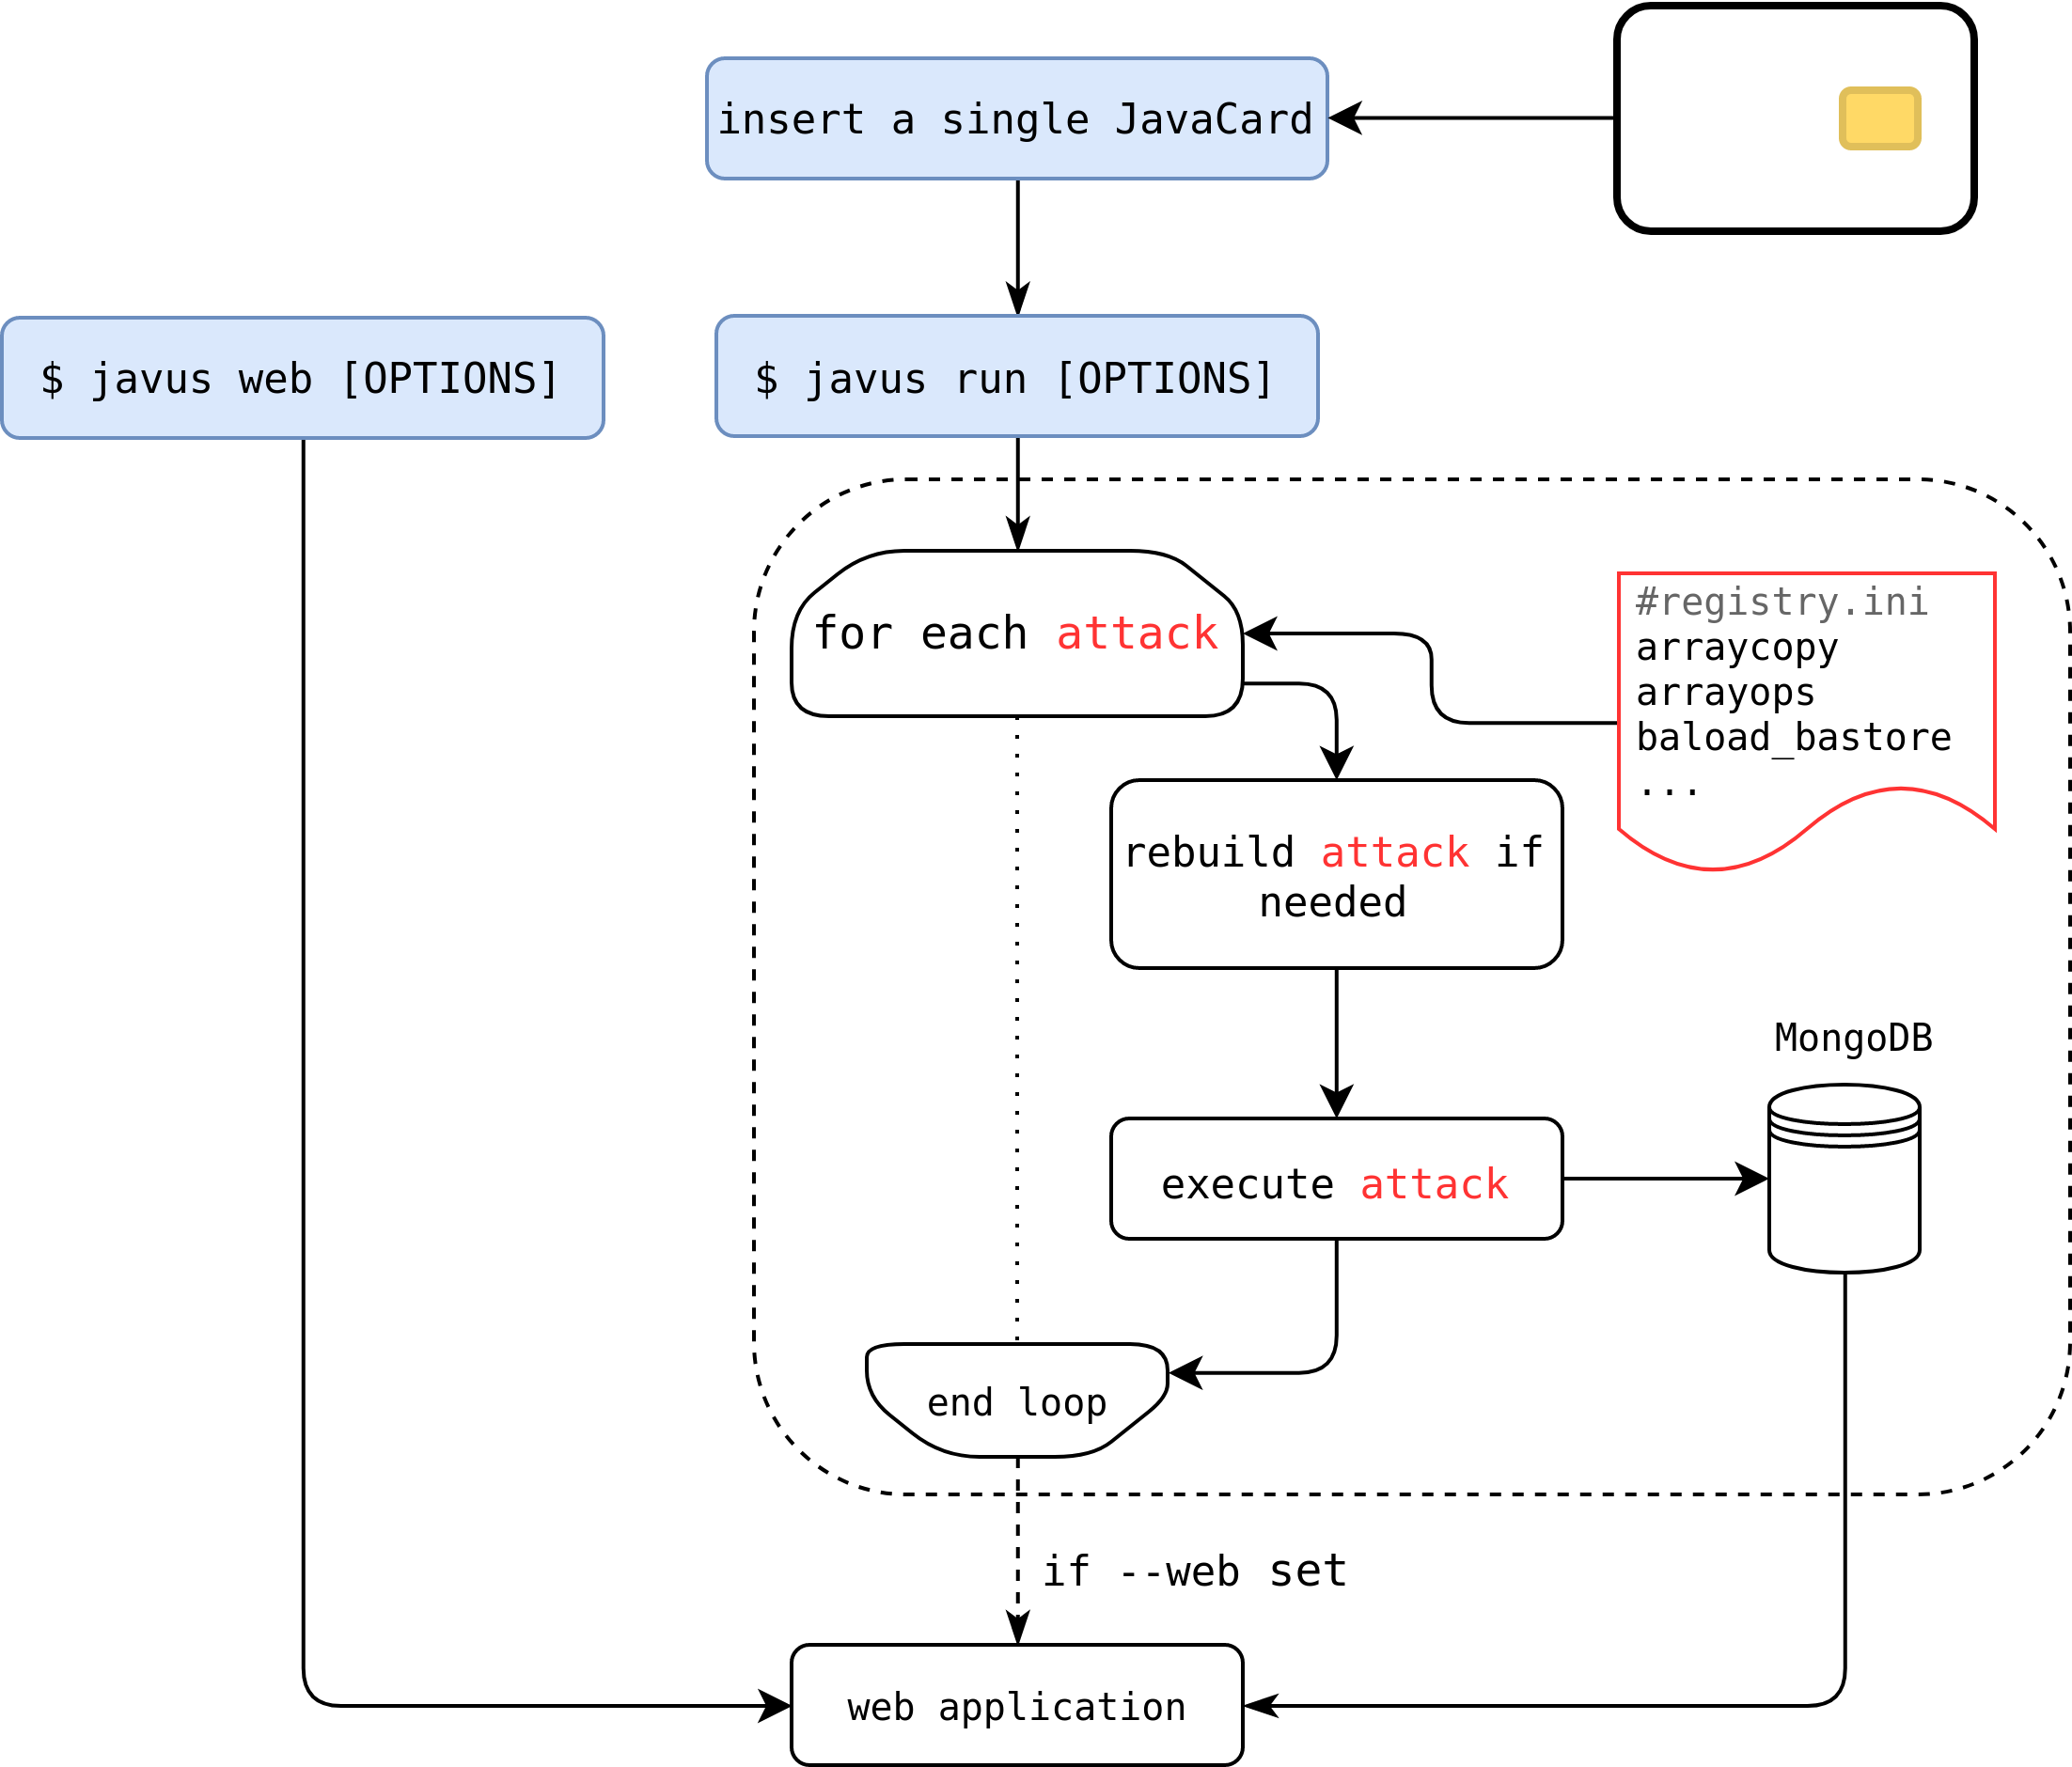
\includegraphics[width=.9\textwidth]{src/diagrams/full-design-new.png}
        \caption{High-level diagram of the run of the application. The part with the dashed rectangle is visualized in more detail in the figure~\ref{fig:execute-attack-diagram}.}
        \label{fig:full-design-diagram}
    \end{figure}

        
    Not only the build process can differ with each attack, but also the execution --- naturaly, each attack can consist of multiple stages (e.g. installing different number of CAP files, sending various number of APDUs). We will cover this in more detail in~\ref{sec:attack-recipe}, but for now, we will only explain, how per attack build and execution is implemented.

    After \shortappclass handles the command line arguments it hands the execution over to \mintinline{python}{javus.analyzer.AnalysisManager}, which iterates over the registered attacks (loaded from \filepath{registry.ini}). For each attack \mintinline{python}{AnalysisManager} loads the appropriate subclass of \shortbuilderclass respectively \shortexecutorclass that is responsible for building, respectively executing the attack. Now we will take a closer look at those two classes. While reading the next sections the reader can consult the diagram in the figure~\ref{fig:execute-attack-diagram}.

    % TODO second diagram, change to <attack>
    \begin{figure}[htb]
        \centering
        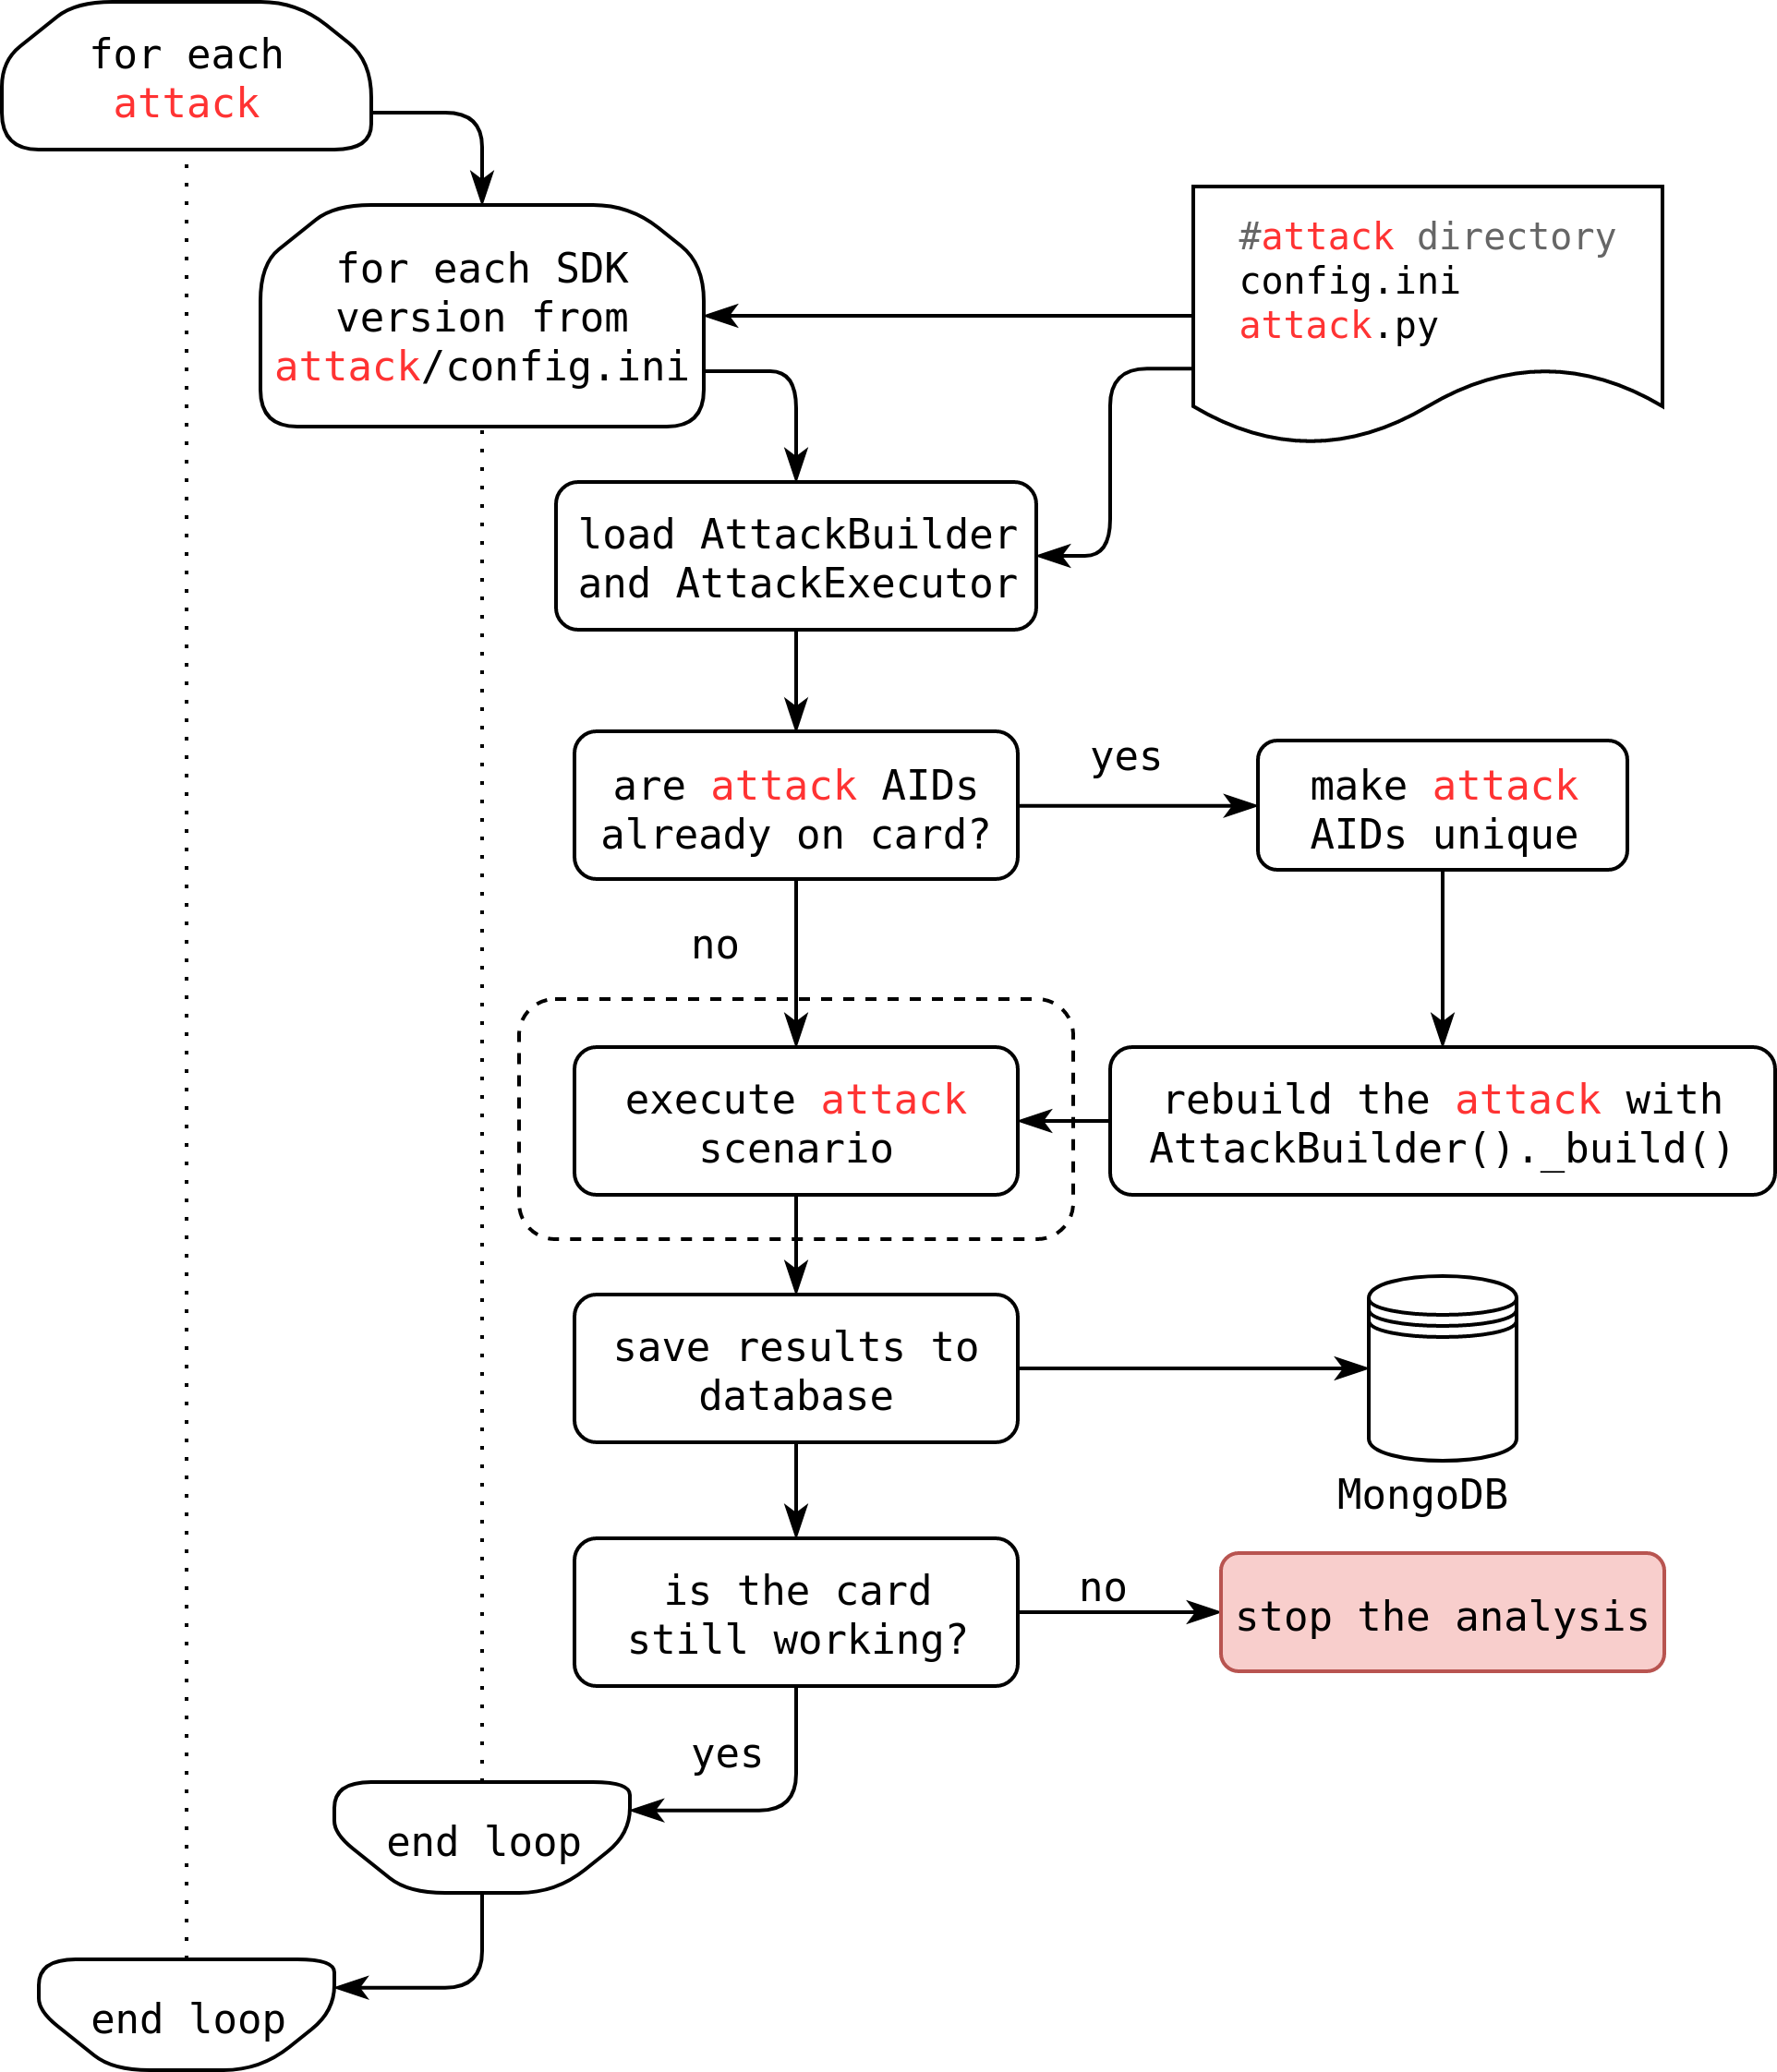
\includegraphics[width=.8\textwidth]{src/diagrams/execute-attack.png}
        \caption{A detailed look at the main attacks execution loop. The final diagram, that fully explains the part in the dashed rectangle is in~\ref{fig:execute-scenario}.}
        \label{fig:execute-attack-diagram}
    \end{figure}



        \subsection{The class \builderclass}\label{subsec:builder-class}
        The ability to build an attack during the run of the analysis means having an automated way of creating all the necessary CAP files, that need to be installed during the attack. Not only creating them but, if the attack requires, also performing any malicious alterations of  e.g.\ the byte code of a particular CAP file (such alteration is necessary for most of the attacks registered in the framework at the moment of writing). Dynamic rebuild of an attack is mainly motivated by the problem of AID uniqueness. In short, an attack would fail before it even started, if any of the AID it was built with is already present on the card (we go into further details in~\ref{sec:uniq-aid}).

        On one hand, attacks naturaly have different build processes (e.g.\ they consists of a different number of packages and applets). On the other hand, some of them might be so similar, that it makes sense for them to share the build process. To allow both we have decided to do the following.
        % To achieve both of those goals, i.e. have the ability to automate the builds while leaving enough room for future attacks, we have decided to do the following.

        To build the CAP files we use Apache Ant. Each attack needs to implement \mintinline{bash}{build.xml} file with a few Ant targets (\ref{subsubsec:ant-targets} discusses the details). The framework provides a class \builderclass, that calls the necesary Ant targets during the runtime. In case a further alteration to the build process is needed the class \shortbuilderclass can be subclassed with the class \attackbuilder and the \mintinline{python}{_build} method can be overridden. If only a single attack needs these changes, it is best to put the implementation of \attackbuilder to \filepath{javus/data/attacks/<attack-name>/<attack-name>.py} (the name of the attack directory and the Python module need to match).
        If, however, the build process is shared by multiple attacks, then the implementation can be added to \filepath{javus/data/attacks/<common-name>.py} (the name can be arbitrary). For the latter case to work it's needed to also add the key value pair \mintinline{ini}{module = <common-name>} to the respective section in \filepath{registry.ini}. There are no real requirements regarding the implementation of \mintinline[breakafter=.]{python}{_build} method. For example, the Security Exploration attacks have a custom Java tool, that is called inside the \mintinline{python}{_build} method (see the file \filepath{javus/data/attacks/security_explorations.py} or~\ref{app:sec:sebuilder} for details).

        The last thing we will mention here is, that each attack can also parametrized by JavaCard SDK version (loaded from \filepath{javus/data/attacks/<attack-name>/config.ini}), that means it can built and executed for several SDKs. As the reader will see in the last chapter, the results differ with SDK version significantly.

        \subsection{The class \executorclass}\label{subsec:executor:class}
            For the execution of a single attack scenario we have implemented the class \mintinline{bash}{BaseAttackExecutor}. This class loads the attack scenario (which is defined simply as \scenario class) during the runtime of the analysis and then executes each stage one by one. The scenario stages are defined as a class level attribute \mintinline{python}{Scenario.STAGES}.

            The class \scenario is loaded from \filepath{javus/data/attacks/<attack-name>/<attack-name>.py} module. For most attacks the scenario needs the same type of stages --- they need to install CAP file(s), send some APDUs and uninstall the original files. The class \shortexecutorclass does implement all of these with its methods \stageinstall, \stagesend,\\ \stageuninstall. Each stage also has a \mintinline{python}{_pre_<stage-name>} method, that can perform setup and, more importantly, \mintinline{python}{_assess_<stage-name>}, that determines, whether the stage was successful or not. For example, the \mintinline{python}{_install} stage is by default successful, if an applet is installed without any errors. The stage \mintinline{python}{_send} is by default successful if the APDU response status word is \mintinline{python}{0x9000}. As there is more to scenario and stages we refer the reader to ~\ref{subsec:scenario:definition}, where also the diagram~\ref{fig:execute-scenario} is described.

        The stages \mintinline{python}{_install} and \mintinline{python}{_send} can be used multiple times. With this feature the default stages should cover the needs of common logical attacks. Otherwise, the user can implement their own stage. Similarly to the usage of \shortbuilderclass, the user will then need to subclass \shortexecutorclass with the class \attackexecutor and implement the desired stage methods (also the default methods can be reimplemented). The source code can either be put in \filepath{javus/data/attacks/<attack-name>/<attack-name>.py} or \filepath{javus/data/attacks/<common-name>.py} (in case it will be reused for multiple attacks). How to add a custom stage is explained in more detail in ~\ref{subsubsec:custom-stage} on a concrete example.

        It is important to understand, that only a single \attackbuilder and \attackexecutor is loaded for each attack. The \mintinline{python}{AnalysisManager} first looks for those classes inside the \mintinline{python}{<attack-name>.py} module file inside the attack directory, then in the common module \filepath{javus/data/attacks/<common-name>.py} (that has to be set in the \filepath{javus/data/registry.ini}). Finaly, the manager defaults to \shortbuilderclass or \shortexecutorclass respectively.

    % \subsection{Analysis data gathering and results visualization}
        \section{Results collection and visualization}\label{sec:visualization}
        The goal of the testing framework is to lift as much weight off the shoulders of the user of JavaCards as possible. With \projectname the user only needs to insert a JavaCard and invoke the framework (more on this topic in~\ref{sec:invocation}). After the analysis is done a simply statement, whether the JavaCard is vulnerable or not is not enough. Therefore we made it possible to track many different values about the attacks during the analysis run. The way data about the run are collected makes it possible for the user to specify, which additional values she'd like to track (with some limitations). Due to the nature of the JavaCard environment, each run of the analysis might be unique. Generally, re-running the analysis can yield different results --- not necessarily due to the JCVM reacting differently to the attacks. We don't have means to clean the card complete of the results of the previous attacks. This motivates saving all the data generated by one run of the analysis together as one entry.

        %More realistic reason is e.g.\ the memory of the JavaCard being filled up by the previous analysis run (imagine the case, where the attack applets and packages can no longer be uninstalled).

        Comparing different runs, e.g. comparing results of one attack across multiple JavaCards, is also of interest. This suggests to use more elaborate data storage such as a database. However, instead of using a traditional relational SQL database, we will do with a NoSQL one, MongoDB in particular (more in~\ref{subsubsec:mongodb}). Coming up with general SQL scheme, that could cover all the needs of future attacks would be an issue. Using NoSQL database gives us the freedom not to worry about the relations between JavaCards, attacks, runs, etc. Instead, we can think in terms of \textit{key:value} pairs. Using the MongoDB terminology, each run of the analysis is saved as a new document. The top-level keys in this document are e.g.\ \mintinline{text}{start-time} (a single value, the timestamp of the start of the run) or \mintinline{text}{analysis-results} (its value contains many nested \texttt{key:value} pairs, that hold the results from all the attacks and their stages). This feature also allows the user to save a new value about the attack, that is not tracked by default (see~\ref{subsubsec:custom-stage} for more). In case the reader is not familiar with NoSQL, but is familiar with Python, he can think of the stored data as some huge (nested) Python dictionary. One more way is to see the stored data as a one big JSON object.
        % FIXME We refer the reader to~\ref{} for example of stored data.
      
        % \subsubsection{Manually inspection}
        % FIXME update the picture!
        Storing a lot of data about the runs makes it then naturally harder to present them in a human readable way. For this purpose we have equiped the framework with a custom web page. (The web interface can be seen in figure Appendix~\ref{fig:web-interface-pic}.) The web page allows the user to select previous runs, select a particular attack and display its execution from all of the runs or select a particular card and show the results of all the attacks. 

        % FIXME unknown stage??
        Each attack is then presented with the results from all of its stages. The stages are marked according to their result, which can or cannot be successful, skipped or unknown. A stage is skipped if it does not make sense to execute it. For example, a send stage is skipped if the applet for this stage was not installed successfully. The marks are explained later, when we will use them to present the results~\ref{tab:stage-legend}.
        % This page presents basic information about the run and about the JavaCard tested in that particular run. Then it shows a list of all the attacks, that were executed. Simple marks give an overview of how the attack progressed (see the legend for the marks in~\ref{fig:stage-legend}).
            To view detailed information about a specific stage one can simply click on the stage and more information will be displayed (see the figure~\ref{fig:web-stage-detail}).

    % The user can view the older runs by selecting them from the drop-down list.

    The web interface can be invoked right after the analysis is done by passing the \mintinline{bash}{--web} flag to \mintinline{bash}{javus run} command. Another option is to only start the local webserver with \mintinline[breaklines]{bash}{javus web [--host HOST] [--port PORT]} and view the previously collected results.
        % \subsubsection{Automatic inspection}
    It is of course also possible to connect to the MongoDB directly or through e.g.\ Python and analyze the results in an automated fashion.
            
% \subsection{Cross-platform}




% Command line utility \javus
%     - builder - responsible for building the files needed for the attack
%     - executor - responsible for running the attack
%     - gppw wrapper - responsible for handling communication with the card
%     - mongo DB - responsible for storing the run related data


% TODO move somewhero elso
    \section{Issues encountered during the development of \javus}
        In the next two section we will cover some of the problems, that we had to deal with during the development of the testing framework.
        
        \subsection{The uniqueness of the Application IDentifier}\label{sec:uniq-aid}
        During the development of the framework we have noticed, that after the execution of some attacks on particular cards (for example see the results for \texttt{arraycopy} attack in~\ref{subsec:result-arraycopy}) the applets installed for the purposes of the attack could not be uninstalled anymore (using the \mintinline{bash}{--uninstall} or \mintinline{bash}{--delete} flags of GlobalPlatformPro nor by direct APDU commands for package and applet uninstallation~\ref{sec:jc:lifecycle}). Therefore we could not easily reuse the applet or package AID for another run of the same (or different) attack.

        Similarly, we can imagine a generic JavaCard, that is about to be tested, can already have an applet or package with an AID of some applet, that will be installed during the execution of the attacks. We definitely don't want the testing of an attack to fail, because the necessary applets cannot be even installed on the card. And expecting the user to handle the collisions herself is against the idea of a simple to use testing framework envisioned in~\ref{chp:testing-tool}.

            To overcome this problem we have implemented the following solution. Before each attack is installed we inspect the AIDs, that are present on the card and compare them with the AIDs of the attack that is next. If they do not intersect we can proceed with the attack. In case they do intersect we have two options. The first is to inform the user and attempt to uninstall the problematic applets from the card. However, as we have mentioned earlier, this is not always possible. As such, it is not implemented in the current version of the framework.

            The second option is to generate new unique AIDs for the attack and rebuild the whole attack (when this happens can be seen in the diagram~\ref{fig:execute-attack-diagram}). This option has the downside, that each attack might require different implementation of updating the attack AIDs, so that they are unique.
            % (e.g.\ an attack can comprise of multiple different packages and applets and have more than one or two AIDs).
            However, it is not difficult to do so and we will show example of how to do it later in~\ref{subsec:build:compile}.

        \subsection{A \textit{canonical} form of a logical attack}
        % FIXME can be add to the appendix
        Commonly, the goal of a logical attack is to trigger some specific functionality in the JCVM and (optionally) get a response. Since any communication with a JavaCard (excluding means of a physical attacks now) is done through the APDU protocol (even maintanence of applets, such as installation and uninstallation) we could distill any logical attack into a sequence of APDU commands, that is a sequence of bytes. Looking at an attack in such a way gives us a clear representation. This representation might be simplified into kind of a \textit{canonical form}\footnotemark
        \footnotetext{We use the term \textit{canonical form} loosely here, without any definition. We mention it due to certain similarities to the usage of these terms in other fields of computers science and mathematics.}
        by removing all but the exact bytes needed for the attack to succeed. This representation could work in theory, but is less practical, since the specific byte sequence includes information, that varies across the spectrum of real JavaCards. For example, the byte sequence responsible for the installation of applets has to include the AID of the Card Manager. Similarly, the following APDU commands, that might trigger a specific function need to select specific applet on a card first, again, this would require hardcoding the AID into the byte sequence.

            We start to see the shortcomings of representing the logical attacks in this manner. One work around would be some kind of \textit{parametrized} canonical form. That is, some byte sequences would be hardcoded, but before executing the attack we would also define the AID of the Card Manager of the JavaCard we test and also other parameters. This solution would overcome the problems, but still has others. Byte sequences are a good representation for a computer and automation tools, but not for a developer or a researcher. A developer would like to learn, what is actually causing the vulnerability (e.g. know, which function when called with what parameters misbehaves) in order to mitigate it (by for example avoid the function in question completely). Similarly, a researches would have a tough time discovering new gaps in the JCVM implementation, if he were to work only with raw byte sequences.

            For these reasons we have discarded the idea to destile the attacks to the minimal byte sequences and instead keep the complete infrastruture to build the individual attacks.
            % FIXME change the verb remain in previous sentence..
